\subsection{Exciting Antenna Patterns: What's in Figure E9-2?}

\begin{tcolorbox}[colback=gray!10, colframe=black, title=E9B05] What type of antenna pattern is shown in Figure E9-2? 
\begin{enumerate}[label=\Alph*.]
    \item \textbf{Elevation}
    \item Azimuth
    \item Near field
    \item Polarization
\end{enumerate} \end{tcolorbox}

\subsubsection{Concepts and Explanation}

In antenna theory, it's essential to understand the different types of radiation patterns that antennas can produce. The terms 'elevation', 'azimuth', 'near field', and 'polarization' each refer to different characteristics of antenna performance and orientation in space.

\begin{itemize}
    \item \textbf{Elevation Pattern:} This represents the variation in antenna gain with respect to the angle of elevation above the horizon. It is crucial for understanding how well an antenna performs in terms of vertical coverage.
    
    \item \textbf{Azimuth Pattern:} This is the variation of gain with rotation around the antenna, which typically pertains to horizontal coverage.
    
    \item \textbf{Near Field:} This refers to the area close to the antenna where the electromagnetic fields have different characteristics compared to the far field. Near field patterns are less commonly used in typical performance evaluations for communication systems.
    
    \item \textbf{Polarization:} It refers to the orientation of the electric field of the transmitted wave, which can be linear, circular, or elliptical. Polarization impacts the interaction between antennas and affects signal reception and transmission.
\end{itemize}

Identifying the correct pattern shown in Figure E9-2 requires knowledge on how the elevation pattern is typically represented. Elevation patterns are often depicted in a way that emphasizes vertical performance.

\subsubsection{Visual Representation}

If you're familiar with working with patterns, you might need to visualize the elevation pattern. A simplified diagram can illustrate a typical elevation pattern as follows: 

\begin{center}
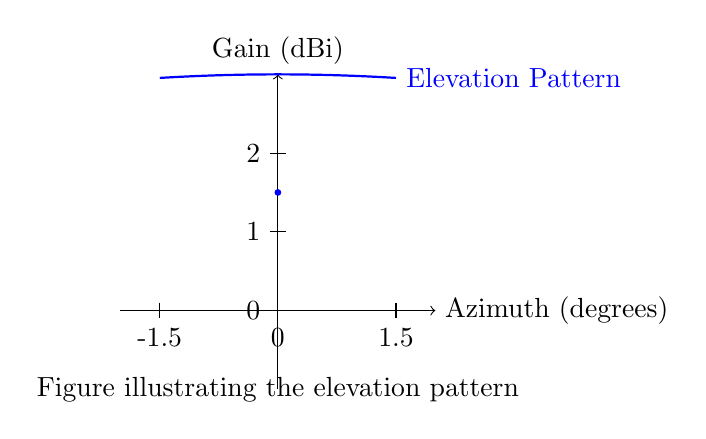
\begin{tikzpicture}
    \draw[->] (-2,0) -- (2,0) node[right] {Azimuth (degrees)};
    \draw[->] (0,-1) -- (0,3) node[above] {Gain (dBi)};
    
    \draw[blue, thick] plot[domain=-1.5:1.5] (\x, {1.5 + 1.5*cos(3*pi*\x)}) node[right] {Elevation Pattern};
    \filldraw[blue] (0,1.5) circle (1pt);
    
    \foreach \x in {-1.5, 0, 1.5} \draw (\x,0.1) -- (\x,-0.1)node[below] {\x};
    
    \foreach \y in {0, 1, 2} \draw (0.1,\y) -- (-0.1,\y)node[left] {\y};
    
    \node at (0, -1) {Figure illustrating the elevation pattern};
\end{tikzpicture}
\end{center}
